\documentclass[12pt]{article}
%\usepackage[document]{ragged2e}
\usepackage{array, amssymb, amsthm, linguex, enumerate, amsmath, physics, enumitem, xcolor, graphicx, xparse}
\let\fg\undefined %remove linguex/siunitx naming clash
\usepackage[english]{babel}
\usepackage[letterpaper,top=2cm,bottom=2cm,left=3cm,right=3cm,marginparwidth=1.75cm]{geometry}
\usepackage[colorlinks=true, allcolors=blue]{hyperref}
\usepackage[group-separator={,}]{siunitx} %\num{12345} -> "12,345"
\usepackage{fancyhdr}
\usepackage{notomath}
\usepackage[T1]{fontenc}

%Number sets
\newcommand{\R}{\mathbb{R}}
\newcommand{\C}{\mathbb{C}}
\newcommand{\N}{\mathbb{N}}
\newcommand{\F}{\mathbb{F}}
\renewcommand{\Re}{\operatorname{Re}}
\renewcommand{\Im}{\operatorname{Im}}
\renewcommand{\L}[1]{\mathcal{L}\left({#1}\right)} %Linear Map

\newcommand{\pmp}{\,\pm\,} %add small extra space to \pm

\NewDocumentCommand{\ceil}{ s m }{% ceiling brackets
    \IfBooleanTF{#1}%
    {\lceil #2 \rceil}% starred: no-autosizing
    {\left\lceil #2 \right\rceil}% unstarred: autosizing
}

\NewDocumentCommand{\ceiling}{ s m }{% ceiling brackets
    \IfBooleanTF{#1}%
    {\lceil #2 \rceil}% starred: no-autosizing
    {\left\lceil #2 \right\rceil}% unstarred: autosizing
}

\NewDocumentCommand{\floor}{ s m }{% floor brackets
    \IfBooleanTF{#1}%
    {\lfloor #2 \rfloor}% starred: no-autosizing
    {\left\lfloor #2 \right\rfloor}% unstarred: autosizing
}

\NewDocumentCommand{\pars}{ s m }{% parenthesis
    \IfBooleanTF{#1}%
    {( #2 ) }% starred: no-autosizing
    {\left( #2 \right) }% unstarred: autosizing
}

\NewDocumentCommand{\inner}{ s m }{% inner product
    \IfBooleanTF{#1}%
    {\langle #2 \rangle}% starred: no-autosizing
    {\left\langle #2 \right\rangle}% unstarred: autosizing
}

\NewDocumentCommand{\innerconj}{ s m }{% inner product
    \IfBooleanTF{#1}%
    {\overline{\langle #2 \rangle}}% starred: no-autosizing
    {\overline{\left\langle #2 \right\rangle}}% unstarred: autosizing
}

\NewDocumentCommand{\brac}{ s m }{% brackets
    \IfBooleanTF{#1}%
    {[#2] }% starred: no-autosizing
    {\left[ #2 \right] }% unstarred: autosizing
}

%default latex bracket size naming
\newcommand{\biggbrac}[1]{\bigg[ {#1} \bigg] }
\newcommand{\bigbrac}[1]{\big[ {#1} \big] }
\newcommand{\Bigbrac}[1]{\Big[ {#1} \Big] }


\RenewDocumentCommand{\over}{ s m }{% fraction 1/arg
    \IfBooleanTF{#1}%
    {\dfrac{1}{#2}}% starred: dfrac
    {\frac{1}{#2}}% unstarred: normal frac
}

\NewDocumentCommand{\pover}{ s m }{% parenthesis around fraction (1/arg)
    \IfBooleanTF{#1}%
    {\left(\dfrac{1}{#2}\right)}% starred: dfrac
    {\left(\frac{1}{#2}\right)}% unstarred: normal frac
}

\NewDocumentCommand{\pfrac}{ s m m}{% parenthesis around fraction (arg1/arg2)
    \IfBooleanTF{#1}%
    {\left( \dfrac{{#2}}{{#3}} \right)}% starred: dfrac
    {\left( \frac{{#2}}{{#3}} \right)}% unstarred: normal frac
}


\newcommand{\Xbar}{\bar{X}}
\newcommand{\Ybar}{\bar{Y}}
\newcommand{\xbar}{\bar{x}}
\newcommand{\ybar}{\bar{y}}


\newcommand{\limn}{\lim_{n\to\infty}}

\newcommand{\gammaDist}[2]{\operatorname{Gamma} \left( {#1},{#2} \right)} %gamma distribution
\NewDocumentCommand{\normalDist}{s g g}{ %normal distibution
    \IfBooleanTF{#1} { % starred, no autosizing parenthesis
      \IfNoValueTF{#2}{ 
          N (\mu,\, \sigma^2 ) %\normalDist* "default" normal distribution N(\mu, \sigma^2)
        } {
            \IfNoValueTF{#3}{N (#2)}{} %\normalDist{arg} --> N(arg)
        }
      \IfNoValueTF{#3}{}{N ( #2, #3 )}  %\normalDist*{arg1}{arg2} --> N(arg1,arg2)
    }  % else (unstarred) autosize parenthesis
    {
        \IfNoValueTF{#2}{
            N \left(\mu,\, \sigma^2 \right) %\normalDist "default" normal distribution N(\mu, \sigma^2)
        } {
            \IfNoValueTF{#3}{N \left(#2\right)}{} %\normalDist{arg} --> N(arg)
        }
        \IfNoValueTF{#3}{}{N \left( #2, #3 \right)} %\normalDist{arg1}{arg2} --> N(arg1,arg2)
    }
}



%colors
\definecolor{ggreen}{RGB}{0, 127, 0}
\definecolor{dgray}{RGB}{63,63,63}
\definecolor{neonorange}{RGB}{255,47,0}
\definecolor{mygray}{rgb}{0.5,0.5,0.5}
\definecolor{eblue}{RGB}{0,74,127}
\newcommand{\red}[1]{\color{red}{#1}\color{black}}
\newcommand{\green}[1]{\color{ggreen}{#1}\color{black}}
\newcommand{\blue}[1]{\color{blue}{#1}\color{black}}
\newcommand{\setRed}{\color{red}}
\newcommand{\setBlack}{\color{black}}
\newcommand{\setBlue}{\color{blue}}
\newcommand{\setGreen}{\color{ggreen}}



\newcommand{\thru}[1]{{#1}_1, \dots, {#1}_n}
\newcommand{\sumThru}[1]{{#1}_1 + \cdots + {#1}_n}
\newcommand{\yn}{Y_1, \dots, Y_n} % Y_1, ..., Y_n
\newcommand{\xn}{X_1, \dots, X_n} % Y_1, ..., Y_n

%hats and tildes
\newcommand{\that}{\widehat{\theta}} % theta hat
\newcommand{\phat}{\widehat{p}} % p hat
\newcommand{\qhat}{\widehat{q}} % p hat
\newcommand{\psihat}{\widehat{\psi}} % psi hat
\newcommand{\Psihat}{\widehat{\Psi}} % Psi hat
\newcommand{\ptilde}{\widetilde{p}} % psi tilde
\newcommand{\Psitil}{\widetilde{\Psi}} % Psi tilde
\newcommand{\betah}{\widehat{\beta}} % beta hat

%2x2 matrix shortcuts
\newcommand{\detx}[4]{\begin{vmatrix}{#1} & {#2}\\{#3}&{#4}\end{vmatrix}} % 2x2 determinant
\newcommand{\bmat}[4]{\begin{bmatrix}{#1} & {#2}\\{#3}&{#4}\end{bmatrix}} % 2x2 matrix brackets
\renewcommand{\pmat}[4]{\begin{pmatrix}{#1} & {#2}\\{#3}&{#4}\end{pmatrix}} % 2x2 matrix parenthesis

%remove any enumerate/itemize indent temporarily
\makeatletter   %% <- make @ usable in macro names
\newcommand*\notab[1]{%
  \begingroup   %% <- limit scope of the following changes
    \par        %% <- start a new paragraph
    \@totalleftmargin=0pt \linewidth=\columnwidth
    %% ^^ let other commands know that the margins have been reset
    \parshape 0
    %% ^^ reset the margins
    #1\par      %% <- insert #1 and end this paragraph
  \endgroup
}
\makeatother    %% <- revert @


\newcommand{\dimrange}[1]{\operatorname{dim}\operatorname{range}{#1}} % dimrange
\newcommand{\dimnull}[1]{\operatorname{dim}\operatorname{null}{#1}} % dimnull
\newcommand{\range}[1]{\operatorname{range}{#1}} %range
\newcommand{\nullspace}{\operatorname{null}} %null

% polynomial notation
\NewDocumentCommand{\poly}{ s g g }{%
    \IfBooleanTF{#1} {
        \IfNoValueTF{#2} {
            \mathcal{P}(\mathbb{R})
        } {
            \mathcal{P}_{#2}(\mathbb{R})
        }
    } {
        \IfNoValueTF{#3} {
            {\mathcal{P}(#2)}
        } { %else
            {\mathcal{P}_{#2}(#3)}
        }
    }
}

\NewDocumentCommand{\bias}{ s m }{% bias(arg)
    \IfBooleanTF{#1}%
    {\operatorname{bias}(#2)}% starred: no autosizing
    {\operatorname{bias}\left(#2\right)}% unstarred: autosizing
}

\NewDocumentCommand{\MSE}{ s m }{% MSE(arg)
    \IfBooleanTF{#1}%
    {\operatorname{MSE}(#2)}% starred: no autosizing
    {\operatorname{MSE}\left(#2\right)}% unstarred: autosizing
}

\NewDocumentCommand{\Var}{ s m }{% variance with parenthesis V(arg)
    \IfBooleanTF{#1}%
    {\operatorname{Var}(#2)}% starred: no autosizing
    {\operatorname{Var}\left(#2\right)}% unstarred: autosizing
}

\NewDocumentCommand{\Varb}{ s m }{% variance with brackets V[arg]
    \IfBooleanTF{#1}%
    {\operatorname{Var}[\,#2\,]}% starred: no autosizing
    {\operatorname{Var}\left[\,#2\,\right]}% unstarred: has autosizing
}

\NewDocumentCommand{\Vb}{ s m }{% another renaming of variance with brackets V[arg]
    \IfBooleanTF{#1}%
    {\operatorname{Var}[\,#2\,]}% starred: no autosizing
    {\operatorname{Var}\left[\,#2\,\right]}% unstarred: has autosizing
}

\NewDocumentCommand{\E}{ s m }{% expectation with parenthesis E(arg)
    \IfBooleanTF{#1}%
    {\operatorname{E}(#2)}% starred: no autosizing
    {\operatorname{E}\left(#2\right)}% unstarred: has autosizing
}

\NewDocumentCommand{\Eb}{ s m }{% expectation with brackets E[arg]
    \IfBooleanTF{#1}%
    {\operatorname{E}[#2]}% starred: no autosizing
    {\operatorname{E}\left[#2\right]}% unstarred: has autosizing
}

\RenewDocumentCommand{\P}{ s m }{% probability with parenthesis Pr(arg)
    \IfBooleanTF{#1}%
    {\Pr (#2) }% starred: no autosizing
    {\Pr \left( #2 \right) }% unstarred: has autosizing
}

\NewDocumentCommand{\prob}{ s m }{% probability with parenthesis Pr(arg)
    \IfBooleanTF{#1}%
    {\Pr (#2) }% starred: no autosizing
    {\Pr \left( #2 \right) }% unstarred: has autosizing
}

\NewDocumentCommand{\eff}{ s m }{% efficiency with parenthesis eff(arg)
    \IfBooleanTF{#1}%
    {\operatorname{eff}(#2)}% starred: no autosizing
    {\operatorname{eff}\left(#2\right)}% unstarred: has autosizing
}

%vertical vector of up to 8 elements
\NewDocumentCommand\vvec{s m g g g g g g g}{%
    \IfBooleanTF{#1} {
        \begin{bmatrix}% if starred use brackets
            \IfNoValueTF{#2}{}{#2}
            \IfNoValueTF{#3}{}{\\#3}
            \IfNoValueTF{#4}{}{\\#4}
            \IfNoValueTF{#5}{}{\\#5}
            \IfNoValueTF{#6}{}{\\#6}
            \IfNoValueTF{#7}{}{\\#7}
            \IfNoValueTF{#8}{}{\\#8}
        \end{bmatrix}
    }  % else (unstarred) use parethesis
    {
        \begin{pmatrix}%
            \IfNoValueTF{#2}{}{#2}
            \IfNoValueTF{#3}{}{\\#3}
            \IfNoValueTF{#4}{}{\\#4}
            \IfNoValueTF{#5}{}{\\#5}
            \IfNoValueTF{#6}{}{\\#6}
            \IfNoValueTF{#7}{}{\\#7}
            \IfNoValueTF{#8}{}{\\#8}
        \end{pmatrix}
    }
}
\def\Cov{\operatorname{Cov}} %Covariance
\def\df{\text{df}} %degrees of freedom

\NewDocumentCommand{\example}{ s g }{% Example header
    \IfBooleanTF{#1}%
    {\vspace{0.1in}}% starred: 0.1in
    {\vspace{0.2in}}% unstarred: 0.2in
    \IfNoValueTF{#2} {\noindent\textbf{\color{eblue} Example: }}{\noindent\textbf{\color{eblue} Example (#2): }}
}
\NewDocumentCommand{\disc}{ s }{% Discussion header
    \IfBooleanTF{#1}%
    {\vspace{0.1in}\noindent\textbf{Discussion: } }% starred: 0.1in
    {\vspace{0.2in}\noindent\textbf{Discussion: } }% unstarred: 0.2in
}
\NewDocumentCommand{\defn}{ s }{% Definition header
    \IfBooleanTF{#1}%
    {\vspace{0.1in}\noindent\textbf{\color{neonorange} Definition: } }% starred: 0.1in
    {\vspace{0.2in}\noindent\textbf{\color{neonorange} Definition: } }% unstarred: 0.2in
}
\NewDocumentCommand{\reason}{ s }{% Reason header
    \IfBooleanTF{#1}%
    {\vspace{0.1in}\noindent\textbf{Reason:} }% starred: 0.1in
    {\vspace{0.2in}\noindent\textbf{Reason:} }% unstarred: 0.2in
}
\NewDocumentCommand{\recall}{ s }{% Recall header
    \IfBooleanTF{#1}%
    {\vspace{0.1in}\noindent\textit{Recall:} }% starred: 0.1in
    {\vspace{0.2in}\noindent\textit{Recall:} }% unstarred: 0.2in
}
\NewDocumentCommand{\remark}{ s }{% Remark header
    \IfBooleanTF{#1}%
    {\vspace{0.1in}\noindent\textit{Remark:} }% starred: 0.1in
    {\vspace{0.2in}\noindent\textit{Remark:} }% unstarred: 0.2in
}

\NewDocumentCommand{\soln}{ s }{% Remark header
    \IfBooleanTF{#1}%
    {\vspace{0.1in}\noindent\textbf{Solution: } }% starred: 0.1in
    {\vspace{0.2in}\noindent\textbf{Solution: } }% unstarred: 0.2in
}

\newcommand{\proj}[2]{\operatorname{proj}_{{#1}}{#2}} %projection
\newcommand{\wideand}{\qquad \text{and} \qquad}

\newcommand{\bu}[1]{\textbf{\underline{{#1}}} } %bold underline
\newcommand{\boldit}[1]{\textbf{\textit{{#1}}} } %bold italix

% put actual quotation marks "around something"
\newcommand{\say}[1]{\textquotedblleft{#1}\textquotedblright}

% max{arg} and min{arg}
\renewcommand{\max}[1]{\operatorname{max}\left\{ #1 \right\}}
\renewcommand{\min}[1]{\operatorname{min}\left\{ #1 \right\}}

%Create a new vspace line no indent
\newcommand{\nl}{\vspace{0.1in}\noindent}
\newcommand{\nnl}{\vspace{0.2in}\noindent}
\newcommand{\nnnl}{\vspace{0.3in}\noindent}
\textwidth=7.02in
\hoffset=-.425in
\begin{document}

\pagestyle{fancy}
\fancyhf{}
\fancyhead[RO]{Matthew Wilder} %header top right
\fancyhead[LO]{MTH 345 - Homework \#1} %header top left
\fancyfoot[CO]{Page \thepage} %page center bottom

\noindent \textbf{Math 345 - Homework 1} \hspace{2.7in} \textbf{Due Monday, September 05, 2022}
\raggedright
\begin{enumerate}
  \item Consider the differential equation $$1 + y^2 + 2(x+1)yy' = 0.$$
\begin{enumerate}
    \item Show that the ODE represents an exact ODE.

\nnl First, since $y' \equiv \displaystyle \dv{y}{x}$, we can rewrite the equation and define functions $M(x,y)$ and $N(x,y)$ as
$$\underbrace{(1+y^2)}_{M}\dd x + \underbrace{2(x+1)y }_{N}\dd y = 0.$$
Then $\displaystyle \pdv{M}{y} = 2y$ and $\displaystyle \pdv{N}{x} = \pdv{x} \pars{2xy+2y} = 2y$. Since $M_y = N_x$, it is an exact ODE. \vspace{.5cm}
    \item Find the general solution to the ODE.

\nnl Continuing with the same $M$ and $N$, integrating these gives
\begin{align*}
    \int M \dd x &= x + xy^2 + C(y) \text{ and}\\
    \int N \dd y &= xy^2 + y^2 + C(x).
\end{align*}
Since $f(x,y) = \int M \dd x = \int N \dd y$, 
\begin{align*}
    & x + xy^2 + C(y) = xy^2 + y^2 + C(x)\\
    \iff & x + C(y) = y^2 + C(x)
\end{align*}
which implies that $C(x) = x$ and $C(y) = y^2$. Hence, the general solution is $f(x,y) = x + xy^2 + y^2 = C$. \vspace{.5cm}
    \item Does a specific solution curve of the ODE pass through the point $(5,0)$? If so, find it.

\nnl Yes, it exists. Evaluating $f(5,0)$ yields $5 = C$. So, substituting this into the general solution gives $f(x,y) = x + xy^2 + y^2 = 5$.
  \end{enumerate}\newpage
  \item \textit{The same but different\dots} Consider the differential equation $$1 + y^2 + 2(x+1)yy' = 0.$$
\begin{enumerate}
    \item Show that the ODE is a separable equation and find the general solution. Justify that this is the same solution found before.

\nnl Rewriting it with leibniz notation and then simplifying,
\begin{align*}
     & \quad (1+y^2)\dd x + 2(x+1)y\; \dd y = 0\\
    \iff & \quad (1+y^2)\dd x = -2(x+1)y\; \dd y\\
    \iff & \quad \frac{1}{-2(x+1)}\dd x = \frac{y}{1+y^2} \dd y\\
    \iff & \quad \int \frac{1}{-2(x+1)}\dd x = \int \frac{y}{1+y^2} \dd y \tag{let $u_1 = x+1, \; u_2 = 1+y^2$}\\
    \iff & \quad \frac{-1}{2} \int \frac{\dd u_1}{u_1} = \frac{1}{2} \int \frac{\dd u_2}{u_2}\\
    \iff & \quad \frac{-1}{2} \ln \abs{u_1} = \frac{1}{2} \ln \abs{u_2} + C_1 \\
    \iff & \quad \frac{-1}{2} \ln \abs{x+1} = \frac{1}{2} \ln \abs{1+y^2} + C_1\\
    \iff & \quad e^{\frac{-1}{2} \ln \abs{x+1}} = e^{\frac{1}{2} \ln \abs{1+y^2} + C_1}\\
    \iff & \quad e^{\ln \abs{(x+1)^{-0.5}}}  = e^{\ln \abs{(1+y^2)^{0.5}}} e^{C_1}\\
    \iff & \quad (x+1)^{-0.5}  = C_2 (1+y^2)^{0.5}\\
    \iff & \quad \frac{1}{\sqrt{x+1}} = C_2 \sqrt{1+y^2}\\
    \iff & \quad \sqrt{1+y^2} \sqrt{x+1} = \frac{1}{C_2}\\
    \iff & \quad (1+y^2)(x+1) = \frac{1}{C_2^2}\\
    \iff & \quad y^2 + xy^2 + x = C\\
\end{align*}
Which is the same as before, $f(x,y) = y^2 + xy^2 + x = C$ \newpage
    \item Use technology and graph the associated slope field. On the picture, sketch the solution curve that passes through the point $(5,0)$.

\noindent (Disclaimer: I have not implemented an ODE solver so the colors are based on the slope field vectors, NOT the vectors of $y$)
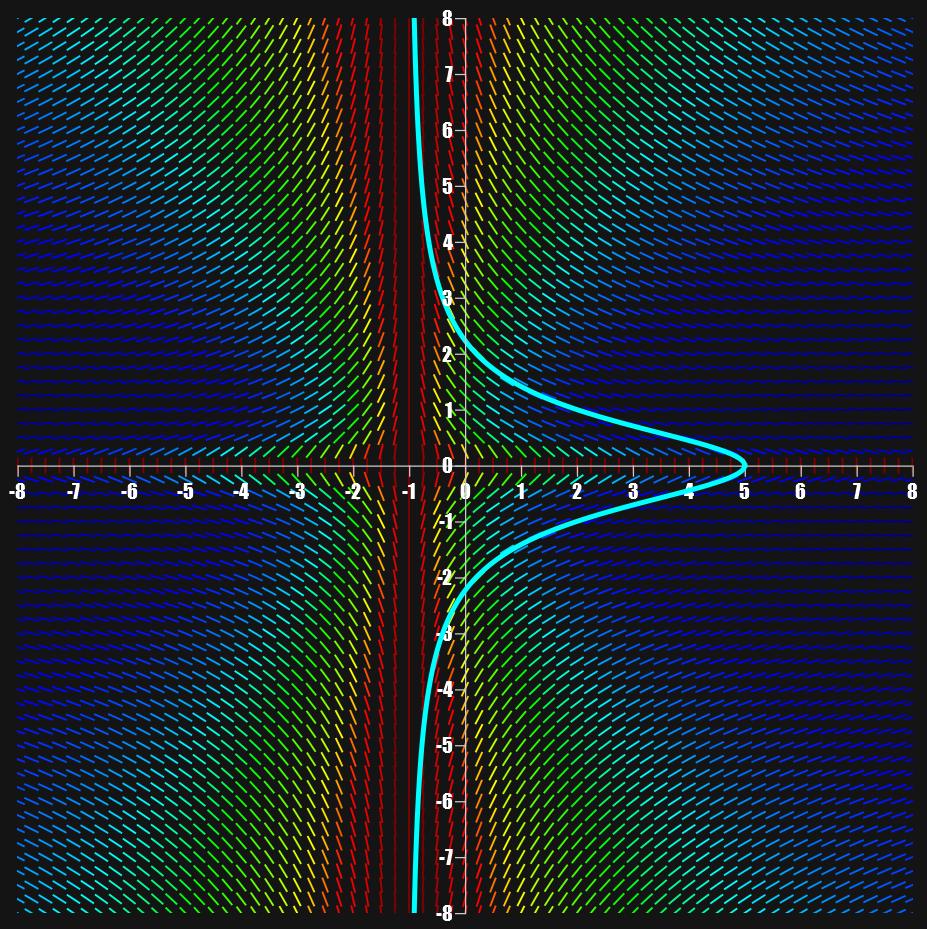
\includegraphics[width=6in]{graph2b.png}
  \end{enumerate}\newpage
  \item For what values of the constants $m,n,$ and $\alpha$ (if any) is the following differential equation exact? $$x^m y^2 y' + \alpha x^3 y^n = 0$$

\nnl Rewriting $y'$ and defining functions $M$ and $N$ gives us 
$$\underbrace{\alpha x^3 y^n}_{M} \dd x + \underbrace{x^m y^2}_{N} \dd y = 0.$$
In order to be exact, we need $M_y = N_x$. Currently $M_y = \alpha x^3 n y^{n-1}$ and $N_x = mx^{m-1}y^2$. To match $y$'s exponents, we need $n-1=2$, which implies $n = 3$. Similarly, to match $x$'s exponents, we need $m-1 = 3$, which implies that $m = 4$. This results in the equation $4x^3y^2 = 3 \alpha x^3 y^2$, further implying that $\alpha = \dfrac43$.

\nl Thus, $n = 3$, $m = 4$, and $\alpha = \dfrac43$ makes this ODE exact.

% There is also the cases where \alpha, n and m are 0 with others varying\vspace{1cm}
  \item Consider the ODE $M(x,y)\dd{x} + N(x,y)\dd{y} = 0.$
\begin{enumerate}
    \item Let $\mu(x,y)$ be a non-vanishing function. What is the relationship between the slope field of the original ODE and the ODE $\mu M \dd x + \mu N \dd y = 0$? Justify your answer.

\nl The slope fields are the same because the equation is being algebraically manipulated with multiplication of the same function on each side. $\mu$ also needs to be non-vanishing to prevent the limits at infinity from being zero where they otherwise wouldn't be. \vspace{.5cm}
    \item Why are the solution curves to the original ODE and the ODE $\mu M \dd x + \mu N \dd y = 0$ identical? Briefly explain.

\nl I believe this is true because integration and derivation are linear operators and can be scaled by scalar functions independent of the differential or integral. This most certainly is not the case for a multivariable $\mu$, but that's why we make $\mu$ independent of one variable, rendering it a function on just one variable.
  \end{enumerate}\vspace{1cm}
  \item Consider the equation $-2xy \dd x + (3x^2 -y^2) \dd y = 0$. 
\begin{enumerate}
    \item Show that the ODE is \textbf{not} exact.

\nnl We define $M$ and $N$ as
$$\underbrace{-2xy}_{M} \dd x + \underbrace{(3x^2 -y^2)}_{N} \dd y = 0.$$
Then $M_y = -2x$ and $N_x = 6x$. Since $M_y \neq N_x$ the ODE is not exact. \vspace{.5cm}
    \item Find an integrating factor that converts the ODE into an exact one.

\nnl To find the integrating factor we will use the formula $\displaystyle \mu = \frac{\mu_x N - \mu_y M}{M_y - N_x}$. From part (a) we have $M, N, M_y, \text{ and } N_x$ so we can do some algebra.
\begin{align*}
    \mu &= \frac{\mu_x N - \mu_y M}{M_y - N_x}\\
    &= \frac{\mu_x (3x^2-y^2) - \mu_y (-2xy)}{-2x - 6x} \tag{substition} \\
    &= \frac{\mu_x (3x^2-y^2)}{-8x} - \frac{\mu_y 2xy}{8x} \tag{linearity}\\
    &= \frac{\mu_x (3x^2-y^2)}{-8x} - \frac{\mu_y y}{4} \tag{like terms}
\end{align*}
From here, we can apply case 2 of integrating factors and let $\mu$ be a function solely in terms of $y$. Consequently, $\mu_x = 0$, so $\mu = \dfrac{-\mu_y y}{4} = \displaystyle \frac{-y}{4}\dv{\mu}{y}$. Now we do some basic calculus to finish finding $\mu$. 
\begin{align*}
    & \quad \mu = \frac{-y}{4}\dv{\mu}{y}\\
    \iff & \quad \frac{1}{y} = \frac{-1}{4 \mu} \dv{\mu}{y} \tag{divide by $\mu y$}\\
    \iff & \quad \frac{1}{y} \dd y = \frac{-1}{4 \mu} \dd{\mu} \tag{multiply by $\dd y$}\\
    \iff & \quad \int \frac{1}{y} \dd y = \int \frac{-1}{4 \mu} \dd{\mu} \\
    \iff & \quad \ln \abs{y} + C = \frac{-1}{4} \ln \abs{\mu}\\
    \iff & \quad \ln \abs{\mu} = -4 \ln \abs{y} = \ln \abs{y^{-4}}\\
    \iff & \quad \mu = y^{-4} + C \tag{$e$ of both sides}
\end{align*}
Letting $C = 0$ gives us a single integrating factor of $\mu = y^{-4}$.\vspace{.5cm}
    \item Using the integrating factor, show that the $\mu$-multiplied ODE is exact.

\nnl Multiplying both sides by $\mu$ yields
$$\underbrace{-2xy^{-3}}_{M} \dd x + \underbrace{(3x^2y^{-4} -y^{-2})}_{N} \dd y = 0.$$
Then $M_y = -2(-3)y^{-4} = -6y^{-4}$ and $N_x = 6xy^{-4}$. Since $M_y = N_x$, the ODE is exact.  \newpage
    \item Find the general solution to the original ODE.

\nl Using the $M$ and $N$ from part (c), integrating for $\int M \dd x$ and $\int N \dd y$ gives
\begin{align*}
    \int M \dd x && \int N \dd y \\
    \int -2xy^{-3} \dd x && \int 3x^2 y^{-4} - y^{-2} \dd y\\
    -x^2 y^{-3} + C(y) && -x^2y^{-3} + y^{-1} + C(x).
\end{align*}
Therefore $C(y) = y^{-1} + C$ and $C(x) = 0$. Hence, $f(x,y) = -x^2y^{-3} + y^{-1} + C$.
This solution can be verified as follows,
\begin{align*}
    & \dv{x} \Bigbrac{ -x^2y^{-3} + y^{-1} = -C} \\
    & 3x^2y^{-4}y' - 2xy^{-3} -y^{-2}y' = 0\\
    & y' = \frac{2xy^{-3}}{3x^2y^{-4}-y^{-2}}\\
    & y' = \frac{2xy^2}{3x-y^2} = \dv{y}{x}\\
\end{align*}
  \end{enumerate}\vspace{0.1in}
  
  \newpage
  \noindent \textbf{\say{Homogeneous} non-linear first-order equations} \vspace{0.1in}
  \item \textit{homogeneous \underline{functions}}

\noindent \textbf{def:} A function $f(x,y)$ is a \textbf{homogeneous function of degree $n$} if given any scalar $\alpha$, $f(\alpha x, \alpha y) = \alpha^n f(x,y)$.

\noindent Determine the degree of homogeneity for the following functions.
\begin{enumerate}
    \item $g(x,y) := x^3 + y^3$
\begin{align*}
    g(\alpha x, \alpha y) &= (\alpha x)^3 + (\alpha y)^3 \\
    &= \alpha^3 x^3 + \alpha^3 y^3\\
    &= \alpha^3 (x^3 + y^3)\\
    &= \alpha^3 f(x,y)
\end{align*}
Therefore $g$ is a homogeneous function of degree 3.
 \vspace{.5cm}
    \item $h(x,y) := \dfrac{-x}{x^2+y^2}$
\begin{align*}
    h(\alpha x,\alpha y) &= \dfrac{-\alpha x}{(\alpha x)^2+(\alpha y)^2} \\
    &= \dfrac{-x}{\alpha x^2+\alpha y^2} \\
    &= \dfrac{-x}{\alpha (x^2 + y^2)}  \\
    &= \alpha^{-1} h(x,y)
\end{align*}
Therefore $h$ is a homogeneous function of degree -1. \vspace{.5cm}
    \item $k(x,y) := \dfrac{y^2 + 2xy}{x^2}$
\begin{align*}
    k(\alpha x, \alpha y) &= \dfrac{(\alpha y)^2 + 2(\alpha x) (\alpha y)}{(\alpha x)^2}  \\
    &= \dfrac{\alpha^2 y^2 + 2\alpha^2 xy}{\alpha^2 x^2} \\
    &= \alpha^0 \dfrac{y^2 + 2xy}{x^2} \\
    &= \alpha^0 k(x,y)
\end{align*}
Therefore $k$ is a homogeneous function of degree 0.
  \end{enumerate}\vspace{1cm}\newpage
  \item Prove the following proposition

\noindent \textbf{Prop:} If $f(x,y)$ is a homogeneous function of degree 0, it can always be expressed as $G(y/x)$ where $G(t)$ is a scalar function of one-variable.

\noindent (Hint: When $x \neq 0,\; f(x,y) = (1/x)^0 f(x,y).$)

\begin{proof}
    For $x \neq 0$, let $\alpha = 1/x$. Then by our assumptions $$f(x,y) = \alpha^0 f(x,y)  = f(\alpha x, \alpha y) = f \pars{\frac{x}{x}, \frac{y}{x}} = f \pars{1, \frac{y}{x}}.$$ Since the first parameter of $f$ is constant we can define a scalar function $G(t)$ using only the second parameter $t = \dfrac{y}{x}$. Then $G(t) = G(y/x) = f(x,y)$.

    \nl For $x = 0$, $G(y/x)$ would be undefined, but $f(x,y) = f(0, y)$ which is a function of just $y$, so $G(t)$ works with $y = t$.
\end{proof}\vspace{1cm}
  \item Prove the following proposition

\noindent \textbf{Prop:} Let $\displaystyle \dv{y}{x} = f(x,y)$ be such that $f(x,y)$ is a homogeneous function of degree 0. Then, through the substitution $u = y/x$, the ODE converts to a separable ODE of the form $$\dv{u}{x} = \over{x} \brac{f(1,u) - u}.$$
(Hint: Differentiate the substitution $u = y/x$ or $y = ux$.)

\begin{proof}
    Using the previous proposition with our hypothesis of degree 0 means that $f(x,y) = f(1,u)$, we will use this substitution later. Let $y = ux$. Differentiating both sides yields $\dd y = x \dd u + u \dd x$ by the product rule. Returning to our original $f(x,y)$ and substituting $\dd y$ with the former gives the desired result.
    \begin{align*}
        &\dv{y}{x} = f(x,y) \tag{ODE assumption}\\
        &\frac{x \dd u + u \dd x}{ \dd x} = f(x,y) \tag{substitution of $\dd y$}\\
        &\dv{u}{x}\cdot x + u = f(x,y) \tag{simplify fraction}\\
        &\dv{u}{x}\cdot x = f(x,y) - u \tag{subtract $u$}\\
        &\dv{u}{x} = \frac{1}{x} \brac{f(x,y) - u} \tag{divide by $x$} \\
        &\dv{u}{x} = \frac{1}{x} \brac{f(1,u) - u} \tag{substitution with previous proposition}
    \end{align*}
\end{proof}\vspace{1cm}
  \item Solve the ODE $\displaystyle \dv{y}{x} = \frac{y^2 + 2xy}{x^2}$.

\soln By \#6(c) we know that $f(x,y):= \frac{y^2 + 2xy}{x^2}$ is a homogeneous function of degree 0. Given these conditions, we can apply the proposition from \#8 to find
\begin{align*}
    &\dv{u}{x} = \over{x} \brac{f(1,u) - u}\\
    &\dv{u}{x} = \over{x} \brac{u^2 + u}
\end{align*} 
Now, using separation of variables yields
\begin{align*}
    &\frac{1}{u^2 + u} \dd u = \over{x} \dd x \\
    &\int \frac{1}{u^2 + u} \dd u = \int \over{x} \dd x \\
\end{align*}
Doing partial fractions on the $u$ integrand gives
$$\frac{1}{u^2 + u} = \frac{1}{u(u+1)} = \frac{A}{u} + \frac{B}{u+1} \iff A(u+1) + Bu = 1 \implies A = 1 \land B= -1.$$
Hence, 
\begin{align*}
    &\int \frac{1}{u} \dd u - \int \frac{1}{u+1} \dd u= \int \over{x} \dd x \\
    & \ln \abs{u} - \ln \abs{u+1} + C = \ln \abs{x}\\
    & \exp \Bigbrac{\ln \abs{u} - \ln \abs{u+1} + C} = \exp \Bigbrac{\ln \abs{x}}\\
    & \frac{Cu}{u+1} = x\\
    & \frac{Cyx^{-1}}{yx^{-1} + 1} = x \tag{substitution of $u = y/x$}\\
    & C yx^{-1} = y + x \tag{multiply by $yx^{-1} + 1$} \\
    & C = \frac{y}{yx^{-1}} + \frac{x}{yx^{-1}} \tag{divide by $yx^{-1}$}\\
    & C = x + \frac{x^2}{y} \tag{simplify}\\
    & \frac{x^2}{y} = C - x \\
    & y = \frac{x^2}{C-x}
\end{align*}
So the general solution to the ODE is $y(x) = \dfrac{x^2}{C-x}$.
\end{enumerate}
\end{document} 